\documentclass[a4paper,12pt]{article}
% \usepackage[utf8]{inputenc}
\usepackage{parskip}
% \usepackage[sorting=none]{biblatex}
% \usepackage{url}
\usepackage{epsfig}
\usepackage{graphics}
\usepackage{fancyhdr}

\usepackage{mathtools}
% \usepackage{graphicx}
\usepackage[justification=centering]{caption}
\usepackage{caption}
\usepackage{subcaption}
\usepackage{amssymb}
\usepackage{amsmath}
\usepackage{tabularx}
\usepackage{xcolor}
\usepackage{multirow}
\usepackage{graphicx}
\usepackage{xcolor}
\usepackage{arydshln}
\usepackage{tikz}
\usetikzlibrary{shapes.geometric, arrows}


\newcommand*{\progName}[1]{\mbox{\texttt{#1}}}

\usepackage{geometry}
\geometry{
  paper=a4paper,
  margin=54pt,
  includeheadfoot
}

% \documentclass{amsart}

% \usepackage[margin=1in]{geometry}        
\usepackage[utf8]{inputenc} % allow utf-8 input
\usepackage[T1]{fontenc}    % use 8-bit T1 fonts
\usepackage{hyperref}       % hyperlinks
\usepackage{url}            % simple URL typesetting
\usepackage{booktabs}       % professional-quality tables
% \usepackage{amsfonts}       % blackboard math symbols
\usepackage{nicefrac}       % compact symbols for 1/2, etc.
\usepackage{microtype}      % microtypography
\usepackage{amsmath,amsfonts,amssymb}
% \usepackage{todonotes}

\usepackage{algorithm}
\usepackage{algpseudocode}

\usepackage[english]{babel}
\newtheorem{theorem}{Theorem}
\usepackage{soul}

\DeclareMathOperator*{\argmax}{arg\,max}
\DeclareMathOperator*{\argmin}{arg\,min}

%package for references
\usepackage[backend=biber, style=alphabetic, sorting=anyt]{biblatex}
\usepackage{csquotes}

\addbibresource{sources.bib}


\title{Collision Avoidance and AI Soccer \\ Assignment 3 Report}

\author{\hspace*{-0.5cm}
GROUP 14\\
\begin{tabular}{cccc}
Shekhar Devm Upadhyay & Linyi Zhang\\
20010531 & 19991218 \\
sdup@kth.se & linyi@kth.se \\
\includegraphics[width=0.2\linewidth]{side_profile.jpg} & 
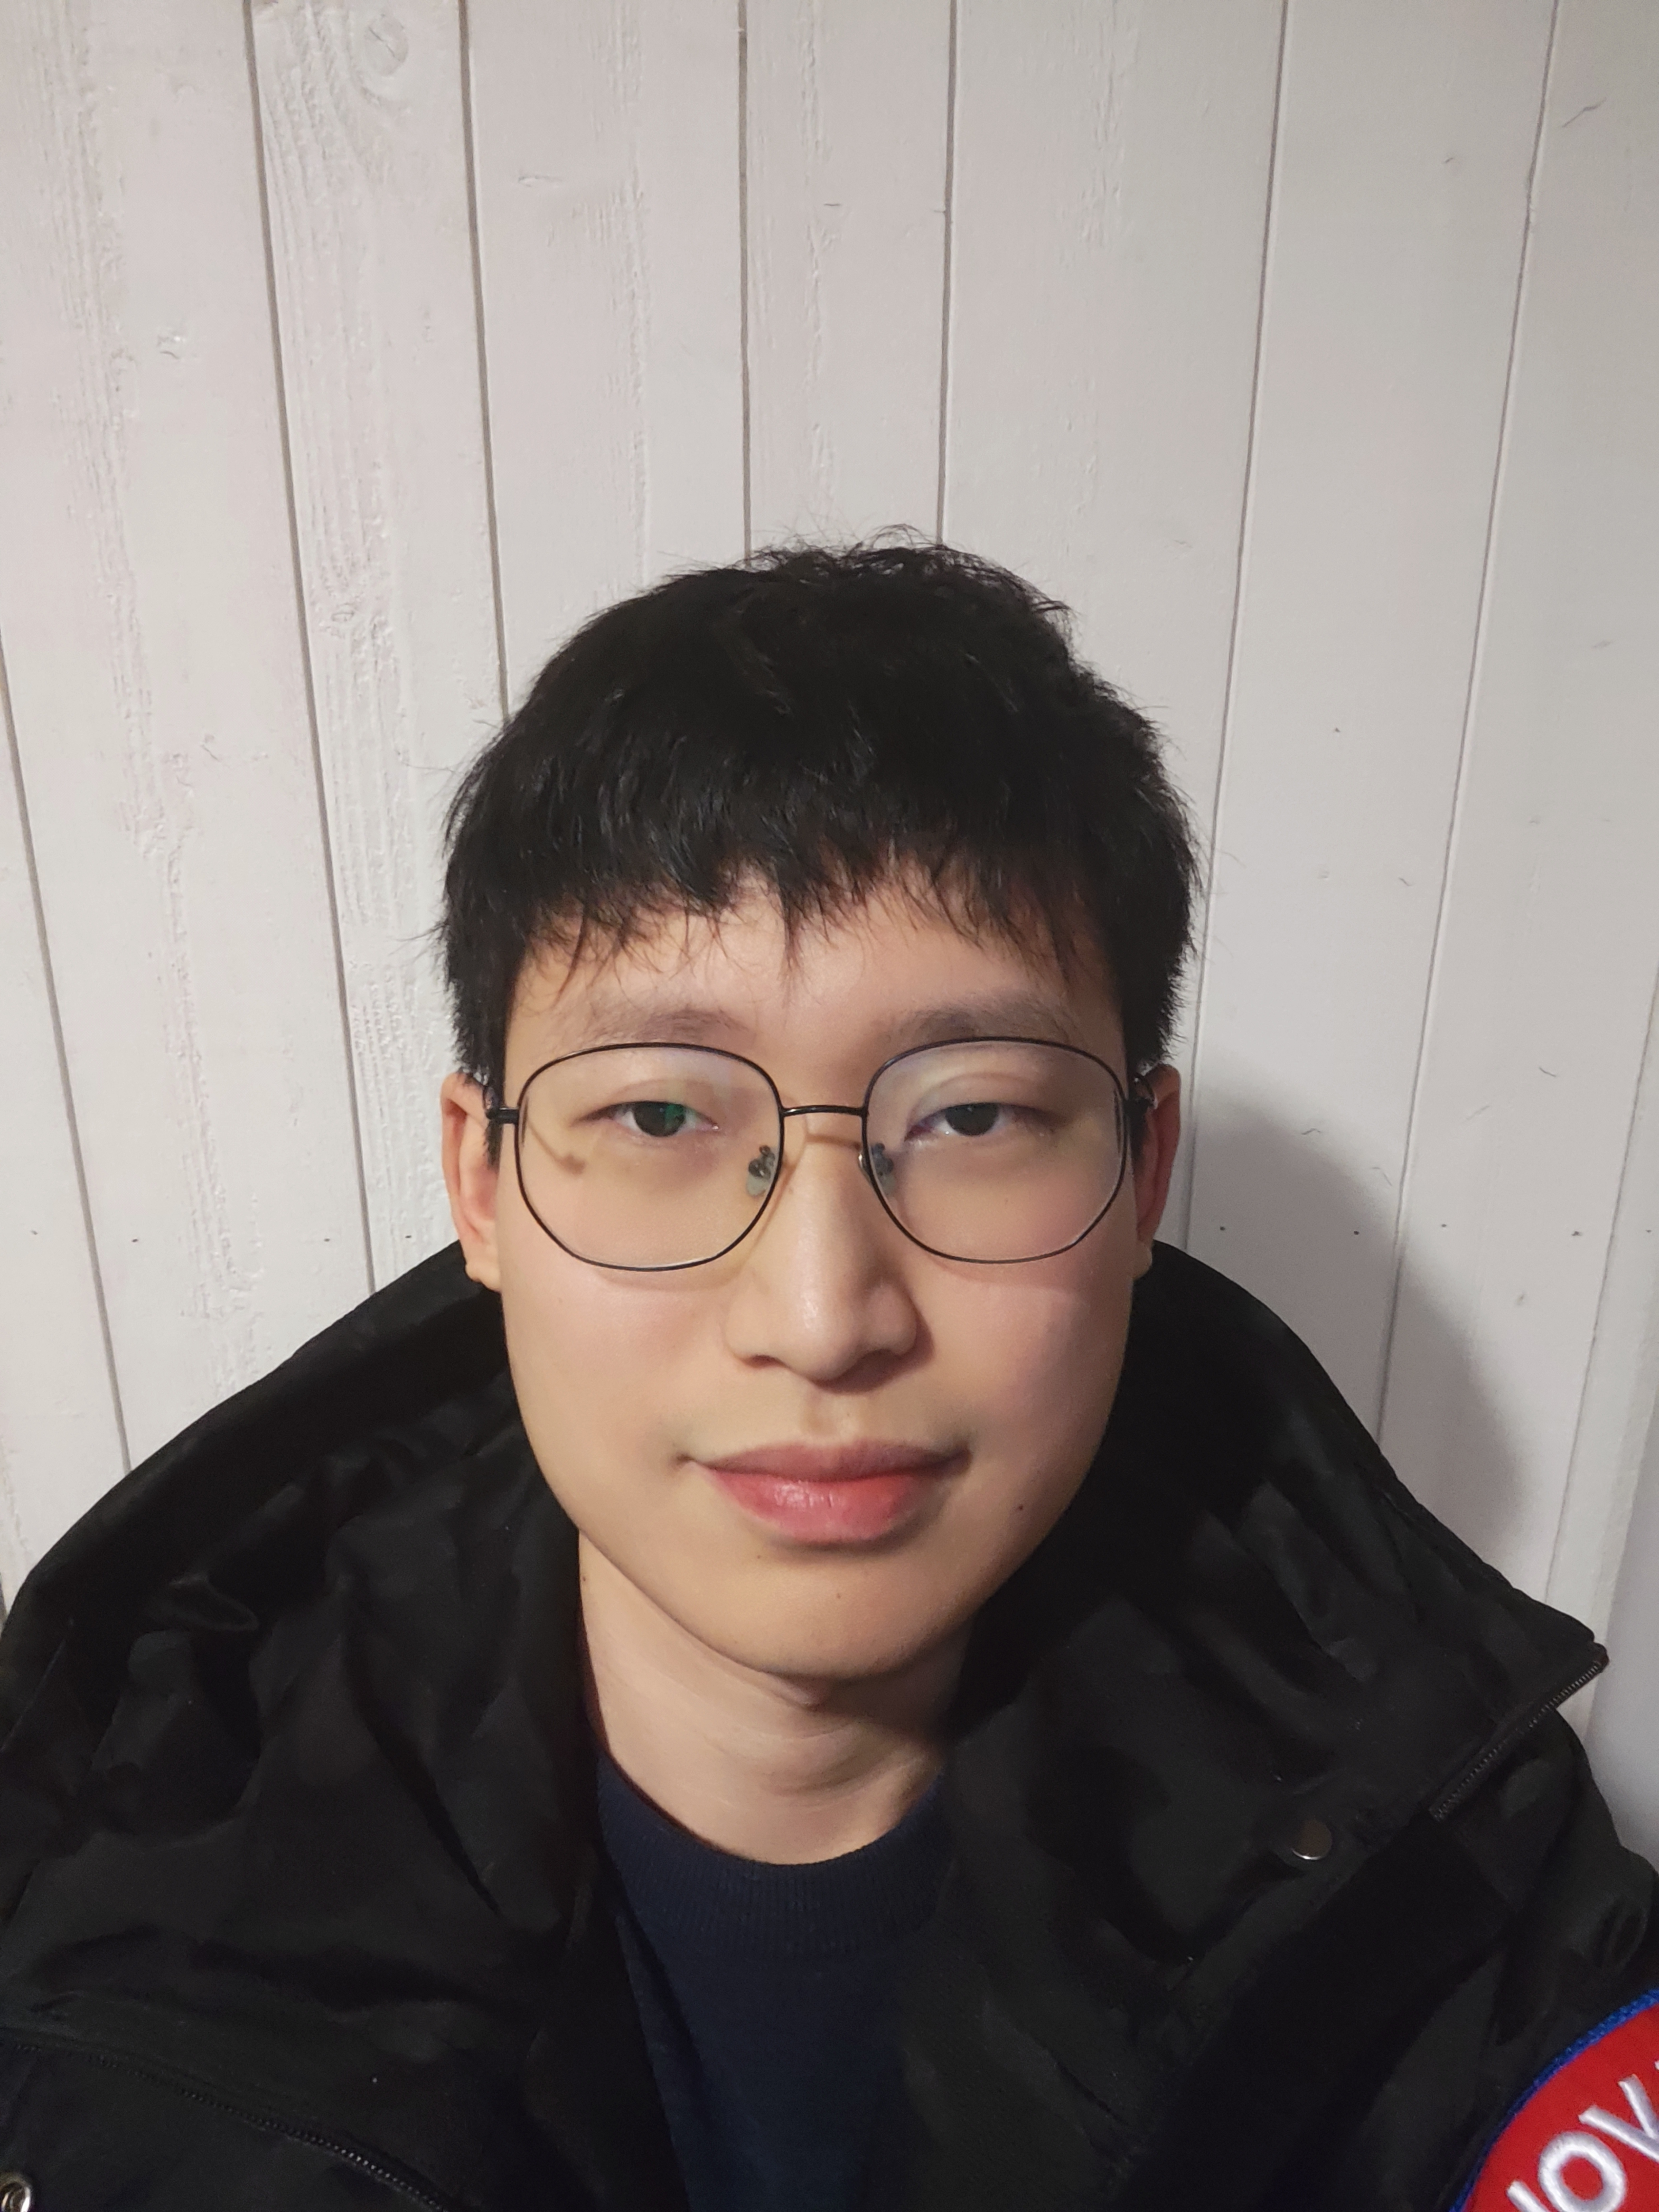
\includegraphics[width=0.17\linewidth]{IMG_20221224_150613.jpg}
\end{tabular}} 
\date{April 2023}

% \pagestyle{fancy}
\setlength{\headheight}{15pt}
\fancyhf{}
\lhead{DD2438} % DO NOT REMOVE!!!!
\rhead{Shekhar Devm Upadhyay, Linyi Zhang} %% UPDATE WITH YOUR NAMES

\addbibresource{sources.bib}

\begin{document}

\maketitle
\thispagestyle{fancy}

\begin{abstract}
% Describe the problem and importance in detail
% why it is important to study

This academic report addresses two significant research problems in Artificial Intelligence: collision avoidance in multi-agent systems and the creation of AI agents for gaming, and presents the respective solutions implemented by the authors based on a comprehensive literature review. 

Collision avoidance is vital in domains such as unmanned aerial vehicles, autonomous vehicles, and mobile robots to ensure safety and mission success. Effective strategies are necessary to operate these systems reliably and safely. Developing AI agents for gaming has potential applications in robotics, sports, and real-world scenarios such as search and rescue, surveillance, and transportation. By solving these problems, researchers can advance machine learning, multi-agent systems, and robotics.


We use a novel force based on Reciprocal velocity obstacles to solve the collision avoidance problem. For the soccer problem, we combine the velocity obstacle methods with the decision tree. Generally, the results show that our solutions are satisfactory compared to other results obtained by the competing groups.

\end{abstract}
\clearpage

%% REMEMBER TO WRITE IN A TOP-DOWN FASHION, STARTING EACH SECTION WITH A SUMMARY. 

\section{Introduction}
% Describe the problem and importance in detail

% introduce collision avoidance problem

% introduce soccer problem

Collision avoidance problem is an important problem in domains such as unmanned vehicles and robotics. It studies how multiple robots can work together with avoiding collisions to achieve goals. 
AI agents for gaming has many applications in various fields. Challenges lie in combination of different strategies and the design of the whole structure.



\subsection{Task Description}

This report will discuss two related but separate problems, and present the respective solutions implemented by the authors. For both problems, the authors developed AI agents to efficiently solve the problems in a Unitiy-based simulation environment using drones and cars (separately) as agents. The problems are as follows:

\begin{itemize}
    \item \textbf{Collision Avoidance}: Given a set of agents and target positions in a given environment, find a set of trajectories for the agents such that they do not collide with each other and reach their target positions in the minimum time. There are fifty agents in the environment, and the agents are drones or cars. The environment is a 2D plane with obstacles.
    
    \item \textbf{Soccer}: Learn to play soccer in a simulated environment, competing against other teams. The ``goal'' is to score as many goals as possible in a fixed time period against the other teams, taking server constraints into account. In our scenario, there are three agents in each team, and the agents are drones or cars.
    
\end{itemize}


These problems and their solutions are addressed in further detail in the following section \ref{rel_work}.




\subsection{Contribution}
% Describe the contribution of the report in detail

In this paper we explore how commonly used velocity obstacle methods can be applied to the collision avoidance problem and the soccer problem in a
simulation environment. We also explore how the collision avoidance problem can be solved with traffic lanes and traffic lights strategies. 
And we combine the velocity obstacle strategies with the behavior tree to solve the soccer problem.



\subsection{Outline}
This work will be divided in multiple sections: Section \ref{rel_work} will discuss the problems in detail, and then the related work which offers some insight to the solutions used in the proposed implementations. Section \ref{method} presents our proposed solution. We started by developing robust strategies for the collision avoidance problem, and then incorporated similar approaches into our soccer agent wherever applicable. 

Finally, Section \ref{sec:experiments_and_results} will discuss our results and present a comparison with the best results obtained by the competing groups, and conclude with a discussion of the benefits and limitations of our and other approaches, and possible future work.

\section{Related Work}
\label{rel_work}
% Describe the related work in detail

This section will discuss the related work in detail. The first part will discuss the collision avoidance problem, and the second part will discuss the soccer problem.

\subsection{Collision Avoidance}
\label{rel_work_collision}

\paragraph{Relevance of the Problem}
Collision avoidance is a critical problem in multi-agent systems, where agents must work together to accomplish tasks in a shared environment, where the actions of one agent may affect the state of the environment and the other agents. In this context, collision avoidance is essential to ensure the safety of agents and the success of the mission. This has applications in various domains, including unmanned aerial vehicles, autonomous vehicles, and mobile robots. In these applications, agents must navigate through dynamic and crowded environments while avoiding obstacles and other agents. Thus, developing effective collision avoidance strategies is critical to the reliable and safe operation of multi-agent systems in real-world applications.

Researchers have proposed several strategies to try to solve this problem. In this section, we review some of the commonly used approaches to collision avoidance in multi-agent systems, to provide some insight into the strategies used in our implementation.

\subsubsection{Potential Fields}
\label{rel_work_collision_potential}

{Potential Fields} is a simplistic yet powerful approach to collision avoidance that was first proposed by O. Khatib\cite{Khatib1986} in 1986. This strategy involves assigning a potential function to each agent, representing the desirability of each location in the environment. The agents then move towards areas of low potential, thereby avoiding collisions. While Potential Fields is simple and easy to implement, it suffers from local minima, where agents may get trapped in undesirable configurations. This problem can be addressed by using a combination of Potential Fields and other strategies, such as Velocity Obstacles.

\subsubsection{Velocity Obstacles}
\label{rel_work_collision_velocity}

{Velocity Obstacles} are another popular approach to collision avoidance, first proposed by R. Fiorini and Z. Shiller\cite{osti_665350} in 1998. This strategy involves calculating the velocity obstacle for each agent, which represents the set of velocities that would result in a collision with other agents. Agents then choose a velocity outside of the velocity obstacle to avoid collisions. Velocity Obstacle is robust and can handle dynamic environments, but it may lead to conservative behavior, where agents move too slowly to avoid collisions.

\subsubsection{Social Force Model}
\label{rel_work_collision_social}

The {Social Force Model} is another approach to collision avoidance, first proposed by D. Helbing and P. Molnar\cite{PhysRevE.51.4282} in 1995. This strategy involves modeling the behavior of agents as if they are influenced by social forces, such as repulsion from other agents and attraction to goals. Agents then adjust their velocities to avoid collisions based on these social forces. Social Force Model can handle complex scenarios, such as crowd dynamics, but it may require significant computational resources to simulate.

\subsubsection{Reciprocal Velocity Obstacles}
\label{rel_work_collision_reciprocal}

{Reciprocal Velocity Obstacles (RVO)} is a recent approach to collision avoidance that was introduced by J. van den Berg et al.\cite{Berg2008ReciprocalVO} in 2008. This strategy is an extension of the Velocity Obstacle method that takes into account the velocity obstacles of all agents in the environment. Agents then choose velocities that avoid collisions with all other agents. RVO is computationally efficient and can handle complex scenarios with many agents, but it may lead to oscillatory behavior and may not always generate the optimal trajectory. The problem of oscillatory behavior was addressed by J. Snape, P. van der Berg, et al. in 2011\cite{Snape2011TheHR} by introducing a new strategy called ORCA, which is an extension of RVO.


% summarize the strategies
% In summary, there are several strategies to address collision avoidance in multi-agent systems, each with its advantages and limitations. Potential Fields, Velocity Obstacle, Social Force Model, Reciprocal Velocity Obstacles, and Model Predictive Control are some of the commonly used approaches that have been proposed by researchers over the years. It is important to carefully select the most appropriate strategy based on the specific requirements of the system and the characteristics of the environment in which the agents operate.

In our implementation, we mainly incorporate two of these strategies to address the collision avoidance problem. We use Potential Fields to avoid collisions with static obstacles such as walls, and use Reciprocal Velocity Obstacles to model a novel force of interaction between agents to maintain collision-free trajectories. This will be discussed in further detail in section \ref{method_collision}.

\subsection{Soccer}
\label{rel_work_soccer}

\paragraph{Relevance of the Problem}
Developing AI agents to play games is a fascinating problem that has been a hot research topic for years. The problem involves creating autonomous agents that can work together to achieve a common goal in a dynamic and uncertain environment. The relevance and significance of this problem can be seen in the potential applications in robotics, gaming, and sports. By solving this problem, we can improve the state of the art in multi-agent systems, machine learning, and robotics. Additionally, it can lead to innovations in autonomous systems, which can be applied in real-world scenarios such as search and rescue, surveillance, and transportation.

We relied on an approach based on a behaviour tree to control cars and drones. A behaviour tree is a tree-like structure that contains nodes that represent actions or conditions. The root node branches down to the tree until the leaf nodes are achieved. The leaf nodes are the base actions that define the behaviours.
The nodes are connected to each other in a hierarchical manner. 

In \cite{ABIYEV2016477}, the design of decision making(DM) algorithm based on behaviour trees and fuzzy obstacle avoidance algorithm for control of
soccer robots are presented. Selector begins with "Shoot Goal" sequence and if it fails, it goes to "Pass" sequence. Move behaviour can be implemented using Run, Walk and Stay.
The rules are: If ball is near and ball speed is low then execute sequence walk. If ball is far away and ball speed is high then execute sequence run. If ball is far away and ball speed is very low then execute sequence stay.
The experiment results demonstrate the effectiveness of proposed algorithms in soccer robot control.

In \cite{6606326}, a novel behaviour tree based control used in decision making processes of robot soccer is proposed.
The most impressive point is passing.
The passing behavior tree first controls two robots using parallel sequences, with the passer and receiver aligned, 
and then the tree checks if the pass is safe. If the ball can be passed, the passer shoots the ball.
Next, the sequence waits for the ball to start moving, and once this happens, 
we again wait for the ball to stop, or for the ball to come within the diameter of the receiver's robot, 
at which point the receiver moves and captures the ball. The use of BT approach allows to model complicated 
situations easily that show advantages of this technique over finite state machines widely
used in robot control\cite{6606326}.



In our implementation, we refer to a part of tree structure from these papers. Our method will be discussed in further detail in section \ref{method_soccer}.




\section{Method}
\label{method}
% Proposed method section explaining what you did in more detail

In this section, we will discuss the proposed solutions to the two problems based on the existing approaches described in section \ref{rel_work}. The first part will discuss the collision avoidance problem, and the second part will discuss the soccer problem.


\subsection{From Drones to Cars}
\label{method_diff}

Since drones were easier to manipulate and can move in any direction freely, we developed our solutions for drones first. This reduced our problem to finding the right ``input'' (acceleration vector) at each update step for the agent. In order to apply the same strategies we used for drones to the situation with cars, all we needed to do was to convert the acceleration vector into a set of inputs for the car. Suppose the acceleration vector is given by $\overrightarrow{\mathbf{a}},$ the unit forward direction of the car is given by $\hat{\mathbf{f}},$ and the unit right direction of the car is given by $\hat{\mathbf{r}}.$ Then the inputs for the car can be calculated as follows:

\begin{eqnarray}
  \label{eqn:car_input}
  \begin{aligned}
    % atan(dot product of a and r)
    \text{steering} &= \arctan(\overrightarrow{\mathbf{a}} \bullet \hat{\mathbf{r}}) \\
    % atan(dot product of a and f)
    \text{gas} &= \arctan(\overrightarrow{\mathbf{a}} \bullet \hat{\mathbf{f}}) \\
    % if magnitude of gas is too small, scale it to 0.2. add a comment about epsilon at the end of the line
    \text{gas} &= \text{gas} \cdot \frac{\epsilon}{\text{min}(|\text{gas}|, \epsilon)} \\
    % \text{brake} &= 0 \\
  \end{aligned}
\end{eqnarray}

A negative gas input is taken as a reverse input. To help the car slow down near turns, we also added a brake input that kicks in if the speed is too high near a turn. We found that with a little bit of fine tuning for the value of $\epsilon,$ this approach allows us to use the same strategies for both drones and cars with minimal changes to the code.

\subsection{Collision Avoidance}
\label{method_collision}

The general outline of our approach is as follows: we first plan a reference trajectory for each agent to its goal, and then use a PD-controller to follow the reference trajectory. We also use an assistive drag force to help the agent follow the reference trajectory. We use a force based on Potential Fields to avoid collisions with static obstacles such as walls, and use Reciprocal Velocity Obstacles to model a novel force of interaction between agents to maintain collision-free trajectories. To further increase structure in our approach, we generate directed lanes on the map to avoid collisions of agents moving in opposite directions. We will discuss each of these components in further detail in this section.

\subsubsection{Reference Trajectory}
\label{method_collision_reference}
Before the agents can start moving, we need to plan a path for each agent to its goal. For this purpose, we plan a path for each agent to its goal using the A* algorithm implemented in previous projects. This path provides a series of checkpoints, which are then used as a reference trajectory for the agent. The agent then uses a PD-controller to follow the reference trajectory. We also continue to use an assistive drag force from previous tasks (shown in Figure \ref{fig:drag_force}) to help the agent follow the reference trajectory. This approach works well for a single agent in an empty environment.

% % figure showing drag
% \begin{figure}[!htbp]
%   \centering
%   \includegraphics[width=0.3\textwidth]{./figures/intelli_drag.png}
%   \caption{Assistive drag force to help the agent maintain its reference trajectory.}
%   \label{fig:drag_force}
% \end{figure}



However, this approach does not take into account the presence of other agents in the environment. Therefore, we need to modify this approach to enable our agents to avoid collisions with other agents.

\subsubsection{Inspiration from Potential Fields}
\label{method_collision_potential}
Building on existing infrastructure from previous tasks, we implemented a potential field based approach to avoid collisions with static obstacles. The potential field is a function that assigns a scalar value to each point in the environment, which represents the `potential' of that point. This is equivalently formulated as a force field, where the force is the negative gradient of the potential field. The repulsive force pushes the agent away from obstacles, and the attractive force pulls the agent towards its goal. 

We use Raycasting to look one second ahead of the agent (moving with the agent's current velocity, $\overrightarrow{\mathbf{v}}$) to detect upcoming collisions. If an obstacle (wall) is found, we note the distance to the obstacle ($d$) and the normal vector of the obstacle at the point of collision ($\hat{\mathbf{n}}$). Using this information, the equivalent force of the potential field is shown in Equation \ref{eq:potential_field}.

\begin{equation}
    \overrightarrow{\mathbf{F}}_{\text{wall}} = \left(\left(\|\overrightarrow{\mathbf{v}}\|_{2} - d\right) \cdot \|\overrightarrow{\mathbf{v}}\|_{2}\right)  \hat{\mathbf{n}}
    \label{eq:potential_field}
\end{equation}

Notice here, that the faster the agent is moving, the stronger the repulsive force. This is because the agent will have less time to react to the obstacle, and therefore needs to be pushed away from the obstacle more strongly. Similarly, the closer the obstacle is to the agent (smaller $d$), the stronger the repulsive force. This is because the agent needs to be pushed away from the obstacle more strongly if it is closer to the obstacle.

We also modeled a couloumbic force of interaction (repulsive) between agents when they got too close to each other, to help them move out of the collision and continue towards their goals.

\subsubsection{Force based on Velocity Obstacles}
\label{method_collision_velocity}

% Motivation for modelling a force of interaction between agents based on Velocity Obstacles

The agents we were working with cannot instantaneously change their velocities, our inputs are only controlling the accelerations of the agents. This means that we cannot simply choose a velocity outside of the velocity obstacle to avoid collisions, as the agents may not be able to change their velocities fast enough to avoid an imminent collision. Additionally, the `allowed' velocities may not even take the agents to their goals. Therefore, we need to model a force of interaction between agents that will allow them to avoid collisions while still moving towards their goals.

Another problem with the vanilla Velocity Obstacles approach is that it doesn't take into consideration that the other agents will also try to avoid collisions. This leads to oscillatory behaviour, due to the asymmetry of the framework. A force of interaction seems to be a better approach, as it allows us to model the fact that the other agents will also try to avoid collisions.

% How we modelled the force of interaction

From the basic framework of Velocity Obstacles, we can find the Velocity cones of disallowed velocities for each agent. If the agent's current velocity is inside one of these cones, then the agent is in danger of colliding with the other agent. However, it is not clear how the agent should accelerate in order to avoid the collision.

To make the modelling process simpler, we assumed that the agents are spherical. We tried to make our modeled force a pairwise force, so that we could simply sum up the forces from all the other agents to get the total force on the agent. For the interaction between two agents, we set up the computations shown in Figure \ref{fig:velocity_obstacle_setup}. We assume that our agent has position vector $\overrightarrow{\mathbf{r}_1},$ current velocity $\overrightarrow{\mathbf{v}_1}$ and a radius $s_1.$ Correspondingly, the other agent has position vector $\overrightarrow{\mathbf{r}_2},$ current velocity $\overrightarrow{\mathbf{v}_2}$ and a radius $s_2.$

% % figure showing velocity obstacle
% \begin{figure}[!hptb]
%   \centering
%   \includegraphics[width=0.3\textwidth]{./figures/VO_repulsion_setup.png}
%   \caption{Velocity Obstacle setup for two agents.}
%   \label{fig:velocity_obstacle_setup}
% \end{figure}

As shown in Figure \ref{fig:velocity_obstacle_calculation}, if the velocity of our agent with respect to the other is inside the cone, these two are in danger of colliding. 

Since the idea is to just push the velocity out of the cone, we want to do so with the least amount of force. Therefore, we want to push the velocity out of the cone in the direction of the closest point on the boundary of the cone. This is shown in Figure \ref{fig:velocity_obstacle_calculation} as the Point of Exit. We then use the vector from the head of the current relative velocity to the Point of Exit (scaled appropriately) as the force of repulsion experienced by our agent. 

To take into account the fact that not all collisions are equally dangerous, we scale the force of repulsion based on time to collision. This is an exponential decay, with collisions happening almost immediately given weightage of $1,$ and collisions happening in the far future given weightage of $0.$

% % figure showing velocity obstacle calculation
% \begin{figure}[!hptb]
%   \centering
%   \includegraphics[width= 0.6\textwidth]{./figures/VO_repulsion_calculation.png}
%   \caption{Calculation for the VO\_Repulsion force between two agents.}
%   \label{fig:velocity_obstacle_calculation}
% \end{figure}


\subsubsection{Order in Chaos}
\label{method_order_in_chaos}

With the above two forces, we were able to get the agents to move towards their goals while avoiding collisions with each other and the walls. However, in crowded regions like an intersection, the agents (particularly cars) kept getting stuck in massive pile-ups. While drones could eventually work their way out of the pile-up, cars were unable to do so because of their inability to move in any direction other than forward. 

We felt the need to augment our effort with better traffic control strategies to avoid such situations. Towards this end, we implemented two main strategies: a) traffic lanes, and b) pseudo-traffic lights.

\paragraph{Soft Traffic Lanes}
The paths generated by A star always consisted of checkpoints that were in the middle of the road. This meant that often, two agents headed in opposite directions would be on the same path, and would collide. To avoid this, we introduced the concept of soft traffic lanes. Based on the direction of the agent, we would shift the checkpoints to the left or right of the road by a certain amount ($\delta$), as shown in Figure \ref{fig:soft_traffic_lanes}. This meant that agents headed in opposite directions would be on different paths, and would not collide, even though they were using the same road. We describe the Lane Generator in more detail in the Appendix.



% % figure showing soft traffic lanes
% \begin{figure}[!hptb]
%   \centering
%   \includegraphics[width= 0.6\textwidth]{./figures/soft_traffic_lanes.png}
%   \caption{Soft traffic lanes.}
%   \label{fig:soft_traffic_lanes}
% \end{figure}

In Figure \ref{fig:soft_traffic_lanes}, the dotted blue line is the original path provided by A star, being traversed by two agents headed in opposite directions. The solid green line is the path after the Lane Generator has been applied to the agent started at the bottom, and the solid red line is the path after the Lane Generator has been applied to the agent started at the top left. The two agents are now on different paths, and will not collide, even though they are using the same road.

\paragraph{Pseudo-Traffic Lights}
More often than not, the pile-ups were caused when agents steered away from their paths to avoid collisions, and ended up blocking the path of other agents. We wanted to avoid agents straying from their paths, and to do so, we introduced the concept of pseudo-traffic lights.

The concept is quite simple: instead of letting agents feel the VO-based repulsion force from other agents in its full glory, we wanted to modify it such that it would only affect their motion along the direction of their path. The approach was to simply take the projection of the total repulsion force along the direction of the path, and use that as the repulsion force. This meant that agents would only be repelled along the direction of their path, and would not stray from it. Figure \ref{fig:pseudo_traffic_lights} shows the idea behind the pseudo-traffic lights. We hoped that with enough number of agents in the simulation, this would emulate the effect of traffic lights, and would help avoid pile-ups.

% % figure showing pseudo traffic lights
% \begin{figure}[!hptb]
%   \centering
%   \includegraphics[width= 0.6\textwidth]{./figures/pseudo_traffic_lights.png}
%   \caption{Pseudo-traffic lights. Note that the repulsion force is only along the direction of the path. So the red car slows down a lot, while the blue car does not decelerate as much. The blue car can pass the intersection before the red car, without steering away from its original path.}
%   \label{fig:pseudo_traffic_lights}
% \end{figure}

\subsection{Soccer}
\label{method_soccer}

The general outline of our approach is as follows: we first build a decision tree for each
agent. Assign three different roles to three agents. And define different behaviors for each role. 
And then we combine velocity obstacles to calculate the best position to move to. 
We will discuss each of these components in further detail in this section.

\subsubsection{Decision Tree}
\thispagestyle{empty}

\tikzstyle{results}=[ellipse ,text centered,draw=black]
\tikzstyle{decisions} =[rectangle, rounded corners,text centered, draw = black]

\tikzstyle{arrow} = [-,>=stealth]
% \begin{center}


\begin{tikzpicture}[node distance=1cm]
\node[decisions](rootnode){CloserThanEnemy or BallIsNotInOurHalfField};
\node[decisions,below of=rootnode,yshift=-0.5cm,xshift=-4cm](rhopoint){closest to the ball};
\node[decisions,below of=rootnode,yshift=-0.5cm,xshift=4.5cm](touchpoint){if can kick};
\node[results,below of=rootnode,yshift=-0.5cm,xshift=0cm](result1){spawn camping};
\node[results,below of=rhopoint,yshift=-0.5cm,xshift=-2cm](attacker){attacker};
\node[decisions,below of=rhopoint,yshift=-0.5cm,xshift=2cm](backup){is last defender};
\node[results,below of=attacker,yshift=-0.5cm,xshift=-2.2cm](result4){goal};
\node[results,below of=attacker,yshift=-0.5cm,xshift=0.6cm](result5){chase the ball};
\node[results,below of=touchpoint,yshift=-0.5cm,xshift=-2cm](result6){make a clearance};
\node[decisions,below of=touchpoint,yshift=-0.5cm,xshift=2.5cm](result7){is last defender};
\node[results,below of=result7,yshift=-0.5cm,xshift=-3cm](result8){goalkeeper};
\node[results,below of=result7,yshift=-0.5cm,xshift=1.2cm](result9){block the ball};
\node[results,below of=backup,yshift=-0.5cm,xshift=0.2cm](result10){goalkeeper};
\node[results,below of=backup,yshift=-0.5cm,xshift=3cm](result11){backup};


\draw [arrow] (rootnode) -- node [left,font=\small] {attack} (rhopoint);
\draw [arrow] (rootnode) -- node [right,font=\small] {defence} (touchpoint);
\draw [arrow] (rootnode) -- node [right,font=\small] {goal} (result1);
\draw [arrow] (rhopoint) -- node [left,font=\small] {yes} (attacker);
\draw [arrow] (rhopoint) -- node [right,font=\small] {no} (backup);
\draw [arrow] (attacker) -- node [left,font=\small] {can kick} (result4);
\draw [arrow] (attacker) -- node [right,font=\small] {no} (result5);  
\draw [arrow] (touchpoint) -- node [left,font=\small] {yes} (result6);
\draw [arrow] (touchpoint) -- node [right,font=\small] {no} (result7);  
\draw [arrow] (result7) -- node [left,font=\small] {yes} (result8);
\draw [arrow] (result7) -- node [right,font=\small] {no} (result9);  
\draw [arrow] (backup) -- node [left,font=\small] {yes} (result10);
\draw [arrow] (backup) -- node [right,font=\small] {no} (result11);  
\end{tikzpicture}

% \end{center}

%describe the behaviour tree above

First, we use positions of the agents and the ball to determine whether we are in the attacking or defending phase. 
If we are in the attacking phase, we check if the agent is the nearest to the ball. 
If it is, then we check if it can kick the ball. If it can, then it kicks the ball towards the goal. 
If it cannot, then it chases the ball. If it is not the nearest to the ball, then one agent becomes the goalkeeper and the third agent becomes the backup. 

If we are in the defending phase, then we check if the agent can kick the ball. If it can, then it makes a clearance. 
If it cannot, then we check if it is the last defender. 
If it is, then it becomes the goalkeeper. If it is not, then it moves to block the ball.

Besides, after the goal, all the agents will go back to their initial positions and the game restarts. Therefore, spawn camping is also considered in our behaviour tree.


\subsubsection{Description of Behaviours}

\paragraph{Ball-chasing Strategy}
\label{method_ball_chasing}
We want our agents to be able to chase the ball and head for a collision with it, in order to kick it. To do this, we make use of Velocity Obstacles once again! Previously, our objective had been to get out of the VO cone. This time, however, we want to get into the VO cone between the ball and the agent. This is because we want to head for a collision with the ball, and the VO cone is the region of space that the ball will occupy in the near future. The setting for this is shown in Figure \ref{fig:soccer_VO_attraction_setting}. The agent is headed towards the ball, and the VO cone is the set of velocities that will lead to a collision with the ball. The agent will try to get into the VO cone, and will eventually collide with the ball. The initial setup for our computations is shown in Figure \ref{fig:soccer_VO_attraction_initial_setup}.

% % figure showing ball chasing
% \begin{figure}[!hptb]
%   \centering
%   \begin{subfigure}[b]{0.45\textwidth}
%     \centering
%     \includegraphics[width=\textwidth]{./figures/soccer_VO_attraction_setup.png}
%     \caption{VO\_Attraction Setting}
%     \label{fig:soccer_VO_attraction_setting}
%   \end{subfigure}
%   ~
%   \begin{subfigure}[b]{0.45\textwidth}
%     \centering
%     \includegraphics[width=\textwidth]{./figures/soccer_VO_attraction_setup_2.png}
%     \caption{VO\_Attraction Initial Setup}
%     \label{fig:soccer_VO_attraction_initial_setup}
%   \end{subfigure}
%   \caption{Setup for our Ball-chasing strategy.}
% \end{figure}

% % figure showing ball chasing
% \begin{figure}[!hptb]
%   \centering
%   \includegraphics[width=0.6\textwidth]{./figures/soccer_VO_attraction_calculation.png}
%   \caption{Final form of the Attraction force.}
%   \label{fig:soccer_VO_attraction_calculation}
% \end{figure}

Based on the above, we compute a force that will attract the agent towards the VO cone, as shown in Figure \ref{fig:soccer_VO_attraction_calculation}. Note that this force tries to kill off the component of relative velocity that is perpendicular to the line joining the agent and the ball. This is because we want the agent to head for a collision with the ball, and not just pass by it. We also pump up the relative velocity along the line joining the agent and the ball, so that the agent can catch up with the ball quickly.

\paragraph{Kick Strategy}
\label{method_kick}
Once the agent has caught up with the ball, it needs to kick it. We want to kick the ball towards a desired goal position, but we also want to avoid kicking it into the path of the opponent. It is important to remember that kicking is different from a force in that it provides an \textbf{impulse} to the ball, instantaneously changing its velocity. A kick vector is basically going to get added to the ball's velocity, and the ball will move in the direction of the resultant velocity.

Once again, Velocity Obstacles come to the rescue: we can try to find the best velocity that we can give the ball, so that it moves towards the goal position, but does not enter the VO cone of the opponent. This time, however, we are free to \textbf{choose} a specific velocity for the ball, since we can give it an impulse. The setting for this is shown in Figure \ref{fig:soccer_kick_setting}. The VO cone of the opponent is shown in red, and the VO cone of the ball is shown in blue. The agent wants to kick the ball in such a way that the ball's VO cone does not intersect with the opponent's VO cone. The initial setup for our computations is shown in Figure \ref{fig:soccer_VO_kick_initial_setup}. The final strategy thus obtained is described in more detail in the Appendix.

% % figure showing ball kicking
% \begin{figure}[!hptb]
%   \centering
%   \includegraphics[width=0.6\textwidth]{./figures/soccer_kick_setup.png}
%   \caption{Player and Ball Positions for kicking the ball.}
%   \label{fig:soccer_kick_setting}
% \end{figure}

% % blank line

% \begin{figure}[!htpb]
%   \centering
%   \includegraphics[width=0.6\textwidth]{./figures/soccer_kick_VO_cones.png}
%   \caption{VO Cones of ball and enemy players, and unsafe zones for kicking the ball.}
%   \label{fig:soccer_VO_kick_initial_setup}
% \end{figure}

% \newpage



\paragraph{Backup Strategy}
The backup is a crucial role in a soccer game.
As shown in figure \ref{fig:soccer_backup}, the agent that has a velocity $v$ is the attacker and two enemies are trying to defend it.
We flip the vector that is from our own goal to the attacker, and add some distance to get the backup position.
By doing this, the backup can be slightly ahead of the attacker, which is benefit for attacking. 
If the attacker fails to make a goal, the backup may be the attacker because it may be closer to the ball and kick the ball at the position where is closer to the goal.


% \begin{figure}[!htpb]
%   \centering
%   \includegraphics[width=0.6\textwidth]{./figures/soccer_backup.jpg}
%   \caption{Backup Strategy for the agent.}
%   \label{fig:soccer_backup}
% \end{figure}

\paragraph{Goalie Strategy}
Basically, the agent that is the closest to our own goal will be the goalie. The goalie will try to stay in the goal area, and will try to block the ball from entering the goal. 
The goalie will also try to kick the ball out of the goal area, if it is inside the goal area. 

We try to use velocity obstacles to calculate the best position for the goalie to block the ball. It performs well in host mode but not in client mode. The performance of our goalie in the host mode can be seen in \href{https://youtu.be/coMNcV3A89g}{here}. And \href{https://youtu.be/5VaNUVcJrpA}{link} shows the performance in the client mode.

Finally, we use a simple goalie strategy that the goalie is always on the line between the goal and the ball. Therefore, it can block the enemy's goal.
This approach is not as good as the velocity obstacle approach in host mode, but it is more stable in client mode on the server.




\section{Experiments and Results}
\label{sec:experiments_and_results}

% mention failure to clear intersection with cars
First, we will describe the experimental setup for the two problems, and then we will present the results for each of the problems separately.

\subsection{Experimental Setup}
\label{subsec:experimental_setup}
% Containing the results of other groups in a table, 
The experimental environment was largely dependent on the problems. Both problems shared a a similar map and obstacle structure, the main difference being the agent objectives, environment sizes, and the fact that we didn't have any obstacles in the soccer environment (except, of course, for the boundaries of the field). For each of the problems, we were to compute and pass a set of inputs to the agents (different based on whether the agent was a car or a drone). The agents moved based on the provided input, and the updated positions and velocities were used in the next timestep to compute the next set of inputs. The agents were also provided with a set of parameters that decided how the different forces were weighted. The parameters were tuned by hand separately for each type of agent, and were not changed during the course of the simulation.

All the solutions for Collision Avoidance were repeatedly tested in the Unity game environment on three terrains: an open field, an intersection, and a random map. The open field was a simple map with no obstacles. The intersection was a map with a crossroad and a few obstacles. The random map was a map with randomly generated obstacles. There were two possible initializations for the positions of the agents: first, in a circular formation, and second, in a random formation. The solutions were tested in the Unity game environment with $50$ agents. Based on performance, the solutions were improved and adjusted in an iterative manner.


\subsection{Results}
\label{subsec:results}
In this section, we summarize the results of our experiments. We first present the results of the Collision Avoidance problem, and then present the results of the Soccer problem. We then go on to discuss the merits and shortcomings of the best solutions from all the groups.

\subsubsection{Collision Avoidance}
\label{subsubsec:collision_avoidance_results}

The completion times of the top 7 groups are shown in Tables \ref{tab:compare_results_soccer_drone} and \ref{tab:compare_results_soccer_car}. Since the drones are easier to move and control, the completion times of the drones are consistently lower than the cars on the same terrains. Our results are largely competitive with the remaining groups. We've managed to complete all drone terrains in reasonable amounts of time, and have managed to complete the car terrains except for the intersection.


% order of groups
% G9
% G13
% G3
% G12
% G10
% G16
% G14

% G3	20.5	21	287	32	30.5	26.5
% G9	29	28.52136	44	46	47	40.78668
% G10	42.8	42.9	64.6	158.42	52.05	69.88
% G12	27.06	27.54	88.66	166.03	47.7	69.23
% G13	34	47	55	47	50	47
% G14	31.3	29.68	79.9	260.15	52.4	60
% G16	59.4	38	141.6	191.5	77.2	70.5
% Best Time	20.5	21	44	32	30.5	26.5

% table comparing results of different groups (drones)

% \begin{table}[!hptb]
%   \centering
%   \begin{tabular}{|c|c|c|c|c|c|c|}
%     \hline
%     \textbf{Terrain} & \multicolumn{2}{|c|}{\textbf{Open Field}} & \multicolumn{2}{|c|}{\textbf{Intersection}} & \multicolumn{2}{|c|}{\textbf{Unstructured}} \\
%     \hline
%     \textbf{Group} & \textbf{Circle} & \textbf{Random} & \textbf{Circle} & \textbf{Random} & \textbf{Circle} & \textbf{Random} \\
%     \hline
%     9 & 29 & 28.52 & 44 & 46 & 47 & 40.78 \\
%     \hline
%     13 & 34 & 47 & 55 & 47 & 50 & 47 \\
%     \hline
%     3 & \color{blue}{20.5} & \color{blue}{21} & \color{red}{287} & \color{blue}{32} & \color{blue}{30.5} & \color{blue}{26.5} \\
%     \hline
%     12 & 27.06 & 27.54 & 88.66 & 166.03 & 47.7 & 69.23 \\
%     \hline
%     10 & 42.8 & 42.9 & 64.6 & 158.42 & 52.05 & 69.88 \\
%     \hline
%     16 & 59.4 & 38 & 141.6 & 191.5 & 77.2 & 70.5 \\
%     \hline
%     \textbf{14} & 31.3 & 29.68 & 79.9 & 260.15 & 52.4 & 60 \\
%     \hline
%     \textbf{Overall Best Time} & 20.5 & 21 & 44 & 32 & 30.5 & 26.5 \\
%     \hline
%   \end{tabular}
%   \caption{Completion Times of the top 7 groups with drones on different terrains.}
%   \label{tab:results_drone_CA}
% \end{table}


Group 3 had the best completion times on all but one terrain for the drones. Their approach was based on modified Reciprocal Velocity Obstacles first introduced by \cite{Snape2011TheHR}, which performed very well with drones, although it did take a lot of time in restricted spaces like the intersection. However, since they spent too much time getting their algorithm to work for drones, they did not have enough time fine-tune their car control and did not perform very well with cars.

Group 9, the best performing drone traffic group, had implemented a spot-capturing algorithm where every agent ``claims'' the grid position just in front of them, based on their intended direction of motion. Agents cannot move into positions that have been claimed by others. This can lead to deadlocks at intersections, which the group resolved by implementing a roundabout system, allowing agents to move synchronously in their desired directions, clearing the intersection in a clockwise manner. This approach worked very well for drones, but was not fine-tuned well enough for cars.

% G13	71	69	158	106	130	70
% G1	111	99	110	108	186	95
% G12	66.62	99.53	193.88	248.76	118.05	130.5
% G2	117.6	129.1	184	208.6	176.1	128.1
% G16	85.8	121.8	349.6	522.5	161.5	132.5
% G11	141.1055	165.303	286.7061	443.0058	247.3884	263.6075
% G14	50.64	70.54	1000	1000	123.36	124.12

% table comparing results of different groups (cars)

% \begin{table}[!hptb]
%   \centering
%   \begin{tabular}{|c|c|c|c|c|c|c|}
%     \hline
%     \textbf{Terrain} & \multicolumn{2}{|c|}{\textbf{Open Field}} & \multicolumn{2}{|c|}{\textbf{Intersection}} & \multicolumn{2}{|c|}{\textbf{Unstructured}} \\
%     \hline
%     \textbf{Group} & \textbf{Circle} & \textbf{Random} & \textbf{Circle} & \textbf{Random} & \textbf{Circle} & \textbf{Random} \\
%     \hline
%     13 & 71 & 69 & 158 & \color{blue}{106} & 130 & \color{blue}{70} \\
%     \hline
%     1 & 111 & 99 & \color{blue}{110} & 108 & 186 & 95 \\
%     \hline
%     12 & 66.62 & 99.53 & 193.88 & 248.76 & \color{blue}{118.05} & 130.5 \\
%     \hline
%     2 & 117.6 & 129.1 & 184 & 208.6 & 176.1 & 128.1 \\
%     \hline
%     16 & 85.8 & 121.8 & 349.6 & 522.5 & 161.5 & 132.5 \\
%     \hline
%     11 & 141.11 & 165.30 & 286.71 & 443.01 & 247.39 & 263.61 \\
%     \hline
%     \textbf{14} & 50.64 & 70.54 & \color{red}{NA} & \color{red}{NA} & 123.36 & 124.12 \\
%     \hline
%     \textbf{Overall Best Time} & 47 & 36 &	110 &	106 &	118.05 &	70 \\
%     \hline
%   \end{tabular}
%   \caption{Completion Times of the top 7 groups with cars on different terrains.}
%   \label{tab:results_car_CA}
% \end{table}

Group 13 picked up where Group 9 left off, and implemented a similar spot-capturing algorithm for cars. They also implemented a roundabout system for cars. Their approach worked very well for cars as well as drones, giving them consistently good performance regardless of the terrain and type of agent. They were the best performing group for cars, and the second best performing group for drones.

Group 1 had the best time on the intersection terrain for the cars. Their strategy was initially based on Velocity Obstacles, but they made an interesting discovery - they didn't actually need dynamic collision avoidance based on VO if they introduced enough order into the system. They implemented a system of trailing and leading nodes being claimed by a car when it was close enough to them, and developed a queing system based on node-claiming for cars to wait for their turn to move. They also implemented a roundabout instead of a crossroads, which helped them avoid collisions. They also checked if the goal position of a car blocked the road for other cars, and if so, they found a safe spot within the goal tolerance for this particular to stay in, moving out of the way of other cars as needed. This was a very interesting approach, and worked very well for cars. They were the second best performing group for cars, overall.

Group 12 had an interesting approach: they implemented a Co-operative A-star algorithm for path planning, encouraging agents to form clusters moving in the same direction, and discouraging them from crossing paths of other agents. This was a reasonably good approach, and led to some interesting planned trajectories. It felt similar to how ants move in a line through the use of pheromones. Their approach yielded good results for both cars and drones; they were the third best performing group for cars, and the fourth best performing group for drones.

One of our biggest shortcomings was that our cars failed to clear the intersection, in both kinds of initial configurations. The main reason for this was a sub-optimal reversing algorithm. We just used Raycasts to look directly ahead from the cars for a fixed length. If a wall was detected, we reversed (straight back) for a set amount of time. This was often excessive, and led to the reversing car crashing into other cars behind it. Group 9 had implemented a more sophisticated reversing algorithm. They had two Raycast ``tentacles'' starting from the car center, looking ahead of the car with a slight angle. If a wall was detected, the car would start reversing until the tentacle was no longer detecting a wall. Based on which tentacle had detected the wall, the car would turn in the opposite direction, and then move forward. This was a much more sophisticated approach, and worked very well for them.

We found another interesting implementation detail in Group 13's work - to facilitate smooth turning, they used PD tracking to control the car, but instead of using the next checkpoint as target position, they took a weighted average of the next 3 checkpoints. This helped them to avoid sharp turns, and made their cars much more stable. This approach is quite reminiscent of the ``charge decay'' introduced by us in the first assignment.


\subsubsection{Soccer}
\label{subsubsec:soccer_results}

For Soccer, we measured the performance of our agents by playing against all the other groups, and through the emergence of intelligent behavior in self-play (for both drones and cars).


% \begin{table}[!hptb]
%   \begin{center}
%   \begin{tabular}{|c|c|c|c|c|c|}
%   \hline
%    & Wins & Home draws  & Away draws & Points  \\ \hline
%   Group 12 & 26	& 2	& 4	& 84  \\ \hline
%   Group 14  & 25	& 3 	& 0 	& 78	 \\ \hline
%   Group 2  & 24 &	2	& 3	& 77 \\ \hline
%   Group 1  & 23	& 2 	& 3	& 74	 \\ \hline
%   Group 20  & 22 &	1	& 3	& 70 \\ \hline
%   \end{tabular}
%   \caption{Performance Comparison between all groups in the car soccer problem.}
%   \label{tab:compare_results_soccer_car}
%   \end{center}
% \end{table}


% \begin{table}[!hptb]
%   \begin{center}
%   \begin{tabular}{|c|c|c|c|c|c|}
%   \hline
%   & Wins & Home draws  & Away draws & Points  \\ \hline
%   Group 12 & 29	& 1	& 4	& 92	\\ \hline
%   Group 18  & 23	& 2	& 3	& 74  \\ \hline
%   Group 10  & 22 &	3	& 4	& 73	 \\ \hline
%   Group 20  & 21 &	3	& 4	& 70 \\ \hline
%   Group 14  & 15	& 4	& 3	&52	\\ \hline
%   \end{tabular}
%   \caption{Performance Comparison between all groups in the drone soccer problem.}
%   \label{tab:compare_results_soccer_drone}
%   \end{center}
% \end{table}
  

As shown in Tables \ref{tab:compare_results_soccer_car} and \ref{tab:compare_results_soccer_drone}, Group 12 stands out in both the car soccer problem and the drone problem, as it has the highest number of wins and points. Their approach uses a combination of Reinforcement Learning and rule-based method. Two reinforcement learning based defenders and one rule-based striker are used in the soccer problem. Self training and trained with rule-based strategy are used in the reinforcement learning process. Training is performed for about $430$ million timesteps.

Their winning streak and impressive defense strategies in both competitions demonstrate the power of Reinforcement Learning.

Group 2 gets the third place in the car soccer problem. They build a behaviour tree for each agent. Their behaviour tree is much more complex than ours.
The most impressive point is that they can use the bounce off the wall for goals and passes.

Group 18 was the first group to use the spawn-camping strategy to score easy goals. We took inspiration from them and also incorporated this strategy in our solution after the pre-final tournament. Spawn camping is a strategy that the agent waits for the ball near the enemy's spawn point.  When the ball is spawned, the agent can get the ball and score easily. In both game scenarios, this strategy is very effective.

%Maybe needs an introduction paragraph


% \begin{figure}[hbtp]
%     \centering
%      \begin{subfigure}[b]{0.49\textwidth}
%         \centering
%         \includegraphics[width=\linewidth]{p1(2).png}
%         \caption{Paths for Problem 1}
%         \label{fig:p1}
%      \end{subfigure}
%      \begin{subfigure}[b]{0.48\textwidth}
%         \centering
%         \includegraphics[width=\linewidth]{P3.png}
%         \caption{Paths for Problem 3}
%         \label{fig:p3}
%      \end{subfigure}
%     \caption{The paths found by the Google OR tools to solve the VRP and Short Range Multi-Agent Search.}
%     \label{p1np3paths}
% \end{figure}



\section{Summary and Conclusions}

In this paper, we present our solutions to the collision avoidance problem and the soccer problem in simulated environments in Unity3D. 
For the collision avoidance problem, we use A* algorithm to create paths first and Velocity Obstacles approach to calculate VO Repulsion force to avoid collision.
In crowded regions like an intersection, we try to simulate the traffic light to control the traffic flow and create soft traffic lanes for vehicles to drive.
For the soccer problem, we use behavior tree to control the agent's behaviour. 
Three roles are assigned to the agent: attacker, backup and goalkeeper. Attacker is the agent that is the closest to the ball. Goalkeeper is the agent that is the closest to our own goal. Backup is the third agent that trys to give an assist to the attacker.
For different behaviors, we use different strategies to control the agent.
Exploit the VO cone to find the best velocity to kick the ball and the best position to chase the ball. 

The overall results are satisfactory. We finished seventh in both the car and drone collision avoidance problem.
We only got the eleventh in the drone soccer game. However, the same strategy is used to solve the car soccer problem, and it did work well.
We were the second in the car soccer game.

% \section{Future Work}


% table with 5 columns
% model | performance | competitive advantage | special features | limitations

% \begin{table}[h]
%     \centering
%     \begin{tabular}{|c|c|c|c|c|}
%     \hline
%     \textbf{Model} & \textbf{Performance} & \textbf{Competitive Advantage} & \textbf{Special Features} & \textbf{Limitations} \\ \hline
%     1 & 1 & 1 & 1 & 1 \\ 
%     \hline
%     2 & 2 & 2 & 2 & 2 \\
%     \hline
%     3 & 3 & 3 & 3 & 3 \\
%     \hline

%     \end{tabular}
%     \caption{Summary of the models}
%     \label{tab:models}
% \end{table}


% \begin{table}[h]
%     \centering
%     \begin{tabular}{|c|c|c|c|c|}
%     \hline
%     \textbf{Model} & \textbf{Performance} & \textbf{Competitive Advantage} & \textbf{Special Features} & \textbf{Limitations} \\ \hline
%     1 & 1 & 1 & 1 & 1 \\ 
%     \hline
%     2 & 2 & 2 & 2 & 2 \\
%     \hline
%     3 & 3 & 3 & 3 & 3 \\
%     \hline

%     \end{tabular}
%     \caption{Summary of the models for soccer}
%     \label{tab:models}
% \end{table}






% \clearpage
% \newpage
\printbibliography

\newpage

\appendix
% print the appendix title on the top of the page
\section{Appendix}

\subsection{Maintaining Reference Trajectory}

% figure showing drag
\begin{figure}[!htbp]
  \centering
  \includegraphics[width=0.3\textwidth]{./figures/intelli_drag.png}
  \caption{Assistive drag force to help the agent maintain its reference trajectory.}
  \label{fig:drag_force}
\end{figure}

\subsection{Velocity Obstacle based Repulsion Force}

% figure showing velocity obstacle
\begin{figure}[!hptb]
  \centering
  \includegraphics[width=0.3\textwidth]{./figures/VO_repulsion_setup.png}
  \caption{Velocity Obstacle setup for two agents.}
  \label{fig:velocity_obstacle_setup}
\end{figure}

% figure showing velocity obstacle calculation
\begin{figure}[!hptb]
  \centering
  \includegraphics[width= 0.6\textwidth]{./figures/VO_repulsion_calculation.png}
  \caption{Calculation for the VO\_Repulsion force between two agents.}
  \label{fig:velocity_obstacle_calculation}
\end{figure}

\subsection{Order in Chaos}

% figure showing soft traffic lanes
\begin{figure}[!hptb]
  \centering
  \includegraphics[width= 0.6\textwidth]{./figures/soft_traffic_lanes.png}
  \caption{Soft traffic lanes.}
  \label{fig:soft_traffic_lanes}
\end{figure}

\paragraph{Lane Generator} The Lane Generator is called before the agents start moving, and it does the following: 
\begin{enumerate}
  \item For each agent, iterate over the set of checkpoints in the path provided by A star.
  \item For each checkpoint that is not the goal position, check the line joining it to the next checkpoint. This is the desired direction of motion for the agent.
  \item Take the cross product of the unit $y$ vector ($\hat{\mathbf{e}}_{y}$) with the desired direction of motion. This gives us the direction of offset for the checkpoint.
  \item Move the checkpoint by $\delta$ units in the direction of offset.
\end{enumerate}


% figure showing pseudo traffic lights
\begin{figure}[!hptb]
  \centering
  \includegraphics[width= 0.6\textwidth]{./figures/pseudo_traffic_lights.png}
  \caption{Pseudo-traffic lights. Note that the repulsion force is only along the direction of the path. So the red car slows down a lot, while the blue car does not decelerate as much. The blue car can pass the intersection before the red car, without steering away from its original path.}
  \label{fig:pseudo_traffic_lights}
\end{figure}


\subsection{Soccer}

% figure showing ball chasing
\begin{figure}[!hptb]
  \centering
  \begin{subfigure}[b]{0.45\textwidth}
    \centering
    \includegraphics[width=\textwidth]{./figures/soccer_VO_attraction_setup.png}
    \caption{VO\_Attraction Setting}
    \label{fig:soccer_VO_attraction_setting}
  \end{subfigure}
  ~
  \begin{subfigure}[b]{0.45\textwidth}
    \centering
    \includegraphics[width=\textwidth]{./figures/soccer_VO_attraction_setup_2.png}
    \caption{VO\_Attraction Initial Setup}
    \label{fig:soccer_VO_attraction_initial_setup}
  \end{subfigure}
  \caption{Setup for our Ball-chasing strategy.}
\end{figure}

% figure showing ball chasing
\begin{figure}[!hptb]
  \centering
  \includegraphics[width=0.5\textwidth]{./figures/soccer_VO_attraction_calculation.png}
  \caption{Final form of the Attraction force.}
  \label{fig:soccer_VO_attraction_calculation}
\end{figure}


% figure showing ball chasing
\begin{figure}[!hptb]
  \centering
  \begin{subfigure}[b]{0.45\textwidth}
    \centering
    \includegraphics[width=\textwidth]{./figures/soccer_kick_setup.png}
    \caption{}
    \label{fig:soccer_kick_setting}
  \end{subfigure}
  ~
  \begin{subfigure}[b]{0.45\textwidth}
    \centering
    \includegraphics[width=\textwidth]{./figures/soccer_kick_VO_cones.png}
    \caption{}
    \label{fig:soccer_VO_kick_initial_setup}
  \end{subfigure}
  \caption{Positions and VO Cones of ball and enemy players, and  unsafe zones for kicking.}
  \label{fig:soccer_kicks}
\end{figure}

% blank line

% \begin{figure}[!htpb]
%   \centering
%   \includegraphics[width=0.5\textwidth]{./figures/soccer_kick_VO_cones.png}
%   \caption{.}
%   \label{fig:soccer_VO_kick_initial_setup}
% \end{figure}

\paragraph{Ball Kicking} We kick the ball using the following strategy: 
\begin{enumerate}
  \item First, compute the VO cones for the ball with respect to all the opponent players (as shown in Figure \ref{fig:soccer_VO_kick_initial_setup}).
  
  \item Find the intersection of the VO cones with the line joining the ball and the desired goal object (either goal or teammate). These define the \textbf{unsafe zones} for kicking the ball.
  
  \item Then, kill the component of ball velocity perpendicular to line joining ball and desired goal object (either goal or teammate).
  
  \item Next, find out how much kicking power you have remaining.
  
  \item If all remaining power can be used to make a kick (outside unsafe zones) by simply adding it to the ball's velocity in the direction of the desired goal object, then do so.
  
  \item Else, reduce kick power along the direction of the desired goal object, till the kick is outside the unsafe zones.

  \item Compare kicks to different goal positions (opponent goal and goal posts, friendly players in better positions to make a goal, etc.) based on kick magnitudes thus obtained, and choose the kick with the highest magnitude.  
\end{enumerate}

\begin{figure}[!htpb]
  \centering
  \includegraphics[width=0.5\textwidth]{./figures/soccer_backup.jpg}
  \caption{Backup Strategy for the agent.}
  \label{fig:soccer_backup}
\end{figure}


% \newpage
\subsection{Results}

% \subsubsection{Collision Avoidance}

\begin{table}[!hptb]
  \centering
  \begin{tabular}{|c|c|c|c|c|c|c|}
    \hline
    \textbf{Terrain} & \multicolumn{2}{|c|}{\textbf{Open Field}} & \multicolumn{2}{|c|}{\textbf{Intersection}} & \multicolumn{2}{|c|}{\textbf{Unstructured}} \\
    \hline
    \textbf{Group} & \textbf{Circle} & \textbf{Random} & \textbf{Circle} & \textbf{Random} & \textbf{Circle} & \textbf{Random} \\
    \hline
    9 & 29 & 28.52 & 44 & 46 & 47 & 40.78 \\
    \hline
    13 & 34 & 47 & 55 & 47 & 50 & 47 \\
    \hline
    3 & \color{blue}{20.5} & \color{blue}{21} & \color{red}{287} & \color{blue}{32} & \color{blue}{30.5} & \color{blue}{26.5} \\
    \hline
    12 & 27.06 & 27.54 & 88.66 & 166.03 & 47.7 & 69.23 \\
    \hline
    10 & 42.8 & 42.9 & 64.6 & 158.42 & 52.05 & 69.88 \\
    \hline
    16 & 59.4 & 38 & 141.6 & 191.5 & 77.2 & 70.5 \\
    \hline
    \textbf{14} & 31.3 & 29.68 & 79.9 & 260.15 & 52.4 & 60 \\
    \hline
    \textbf{Overall Best Time} & 20.5 & 21 & 44 & 32 & 30.5 & 26.5 \\
    \hline
  \end{tabular}
  \caption{Completion Times of the top 7 groups with drones on different terrains.}
  \label{tab:results_drone_CA}
\end{table}

\begin{table}[!hptb]
  \centering
  \begin{tabular}{|c|c|c|c|c|c|c|}
    \hline
    \textbf{Terrain} & \multicolumn{2}{|c|}{\textbf{Open Field}} & \multicolumn{2}{|c|}{\textbf{Intersection}} & \multicolumn{2}{|c|}{\textbf{Unstructured}} \\
    \hline
    \textbf{Group} & \textbf{Circle} & \textbf{Random} & \textbf{Circle} & \textbf{Random} & \textbf{Circle} & \textbf{Random} \\
    \hline
    13 & 71 & 69 & 158 & \color{blue}{106} & 130 & \color{blue}{70} \\
    \hline
    1 & 111 & 99 & \color{blue}{110} & 108 & 186 & 95 \\
    \hline
    12 & 66.62 & 99.53 & 193.88 & 248.76 & \color{blue}{118.05} & 130.5 \\
    \hline
    2 & 117.6 & 129.1 & 184 & 208.6 & 176.1 & 128.1 \\
    \hline
    16 & 85.8 & 121.8 & 349.6 & 522.5 & 161.5 & 132.5 \\
    \hline
    11 & 141.11 & 165.30 & 286.71 & 443.01 & 247.39 & 263.61 \\
    \hline
    \textbf{14} & 50.64 & 70.54 & \color{red}{NA} & \color{red}{NA} & 123.36 & 124.12 \\
    \hline
    \textbf{Overall Best Time} & 47 & 36 &	110 &	106 &	118.05 &	70 \\
    \hline
  \end{tabular}
  \caption{Completion Times of the top 7 groups with cars on different terrains.}
  \label{tab:results_car_CA}
\end{table}


% \subsubsection{Soccer}

\begin{table}[!hptb]
  \begin{center}
  \begin{tabular}{|c|c|c|c|c|c|}
  \hline
   & Wins & Home draws  & Away draws & Points  \\ \hline
  Group 12 & 26	& 2	& 4	& 84  \\ \hline
  Group 14  & 25	& 3 	& 0 	& 78	 \\ \hline
  Group 2  & 24 &	2	& 3	& 77 \\ \hline
  Group 1  & 23	& 2 	& 3	& 74	 \\ \hline
  Group 20  & 22 &	1	& 3	& 70 \\ \hline
  \end{tabular}
  \caption{Performance Comparison between all groups in the car soccer problem.}
  \label{tab:compare_results_soccer_car}
  \end{center}
\end{table}


\begin{table}[!hptb]
  \begin{center}
  \begin{tabular}{|c|c|c|c|c|c|}
  \hline
  & Wins & Home draws  & Away draws & Points  \\ \hline
  Group 12 & 29	& 1	& 4	& 92	\\ \hline
  Group 18  & 23	& 2	& 3	& 74  \\ \hline
  Group 10  & 22 &	3	& 4	& 73	 \\ \hline
  Group 20  & 21 &	3	& 4	& 70 \\ \hline
  Group 14  & 15	& 4	& 3	&52	\\ \hline
  \end{tabular}
  \caption{Performance Comparison between all groups in the drone soccer problem.}
  \label{tab:compare_results_soccer_drone}
  \end{center}
\end{table}

\end{document}
